%% LyX 2.0.0 created this file.  For more info, see http://www.lyx.org/.
%% Do not edit unless you really know what you are doing.
\documentclass[english]{beamer}
\usepackage{mathptmx}
\usepackage[T1]{fontenc}
\usepackage[latin9]{inputenc}
\usepackage{color}
\usepackage{babel}
\usepackage{pdfpages}
\usepackage{amsmath}
\usepackage{amssymb}
\usepackage{graphicx}
\ifx\hypersetup\undefined
  \AtBeginDocument{%
    \hypersetup{unicode=true}
  }
\else
  \hypersetup{unicode=true}
\fi

\makeatletter

%%%%%%%%%%%%%%%%%%%%%%%%%%%%%% LyX specific LaTeX commands.
%% A simple dot to overcome graphicx limitations
\newcommand{\lyxdot}{.}


%%%%%%%%%%%%%%%%%%%%%%%%%%%%%% Textclass specific LaTeX commands.
 % this default might be overridden by plain title style
 \newcommand\makebeamertitle{\frame{\maketitle}}%
 \AtBeginDocument{
   \let\origtableofcontents=\tableofcontents
   \def\tableofcontents{\@ifnextchar[{\origtableofcontents}{\gobbletableofcontents}}
   \def\gobbletableofcontents#1{\origtableofcontents}
 }
 \long\def\lyxframe#1{\@lyxframe#1\@lyxframestop}%
 \def\@lyxframe{\@ifnextchar<{\@@lyxframe}{\@@lyxframe<*>}}%
 \def\@@lyxframe<#1>{\@ifnextchar[{\@@@lyxframe<#1>}{\@@@lyxframe<#1>[]}}
 \def\@@@lyxframe<#1>[{\@ifnextchar<{\@@@@@lyxframe<#1>[}{\@@@@lyxframe<#1>[<*>][}}
 \def\@@@@@lyxframe<#1>[#2]{\@ifnextchar[{\@@@@lyxframe<#1>[#2]}{\@@@@lyxframe<#1>[#2][]}}
 \long\def\@@@@lyxframe<#1>[#2][#3]#4\@lyxframestop#5\lyxframeend{%
   \frame<#1>[#2][#3]{\frametitle{#4}#5}}
 \long\def\lyxplainframe#1{\@lyxplainframe#1\@lyxframestop}%
 \def\@lyxplainframe{\@ifnextchar<{\@@lyxplainframe}{\@@lyxplainframe<*>}}%
 \long\def\@@lyxplainframe<#1>#2\@lyxframestop#3\lyxframeend{%
   \frame<#1>[plain]{\frametitle{#2}#3}}
 \def\lyxframeend{} % In case there is a superfluous frame end

%%%%%%%%%%%%%%%%%%%%%%%%%%%%%% User specified LaTeX commands.
%\usetheme{Warsaw}
\usetheme{Boadilla}
% or ...

\usecolortheme{orchid}
\setbeamertemplate{footline}[text line]{} % makes the footer EMPTY

\setbeamercovered{transparent}
% or whatever (possibly just delete it)

\makeatother

\begin{document}
\setbeamercolor{background canvas}{bg=}






\title[Short Paper Title]{Evaluation of a Scratchpad Template as an Online Database for the
University of Guam Insect Collection}


\author{Aubrey Moore}


\institute{Extension Entomologist\\
Western Pacific Tropical Research Center\\
University of Guam}


\date{Entomological Networks Meeting, 2011}

\makebeamertitle


%\pgfdeclareimage[height=0.5cm]{institution-logo}{institution-logo-filename}

%\logo{\pgfuseimage{institution-logo}}



\AtBeginSubsection[]{

  \frame<beamer>{ 

    \frametitle{Outline}   

    \tableofcontents[currentsection,currentsubsection] 

  }

}



%\beamerdefaultoverlayspecification{<+->}








\lyxframeend{}\section*{Introduction}


\lyxframeend{}\lyxframe{Where the is Guam?}

\begin{center}
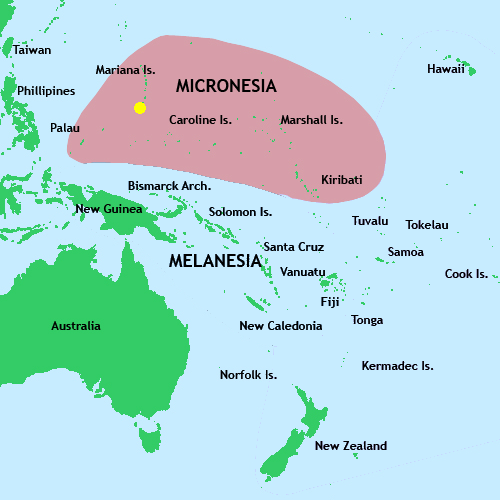
\includegraphics[scale=0.45]{images/Micronesian_Cultural_Area_dot}
\par\end{center}


\lyxframeend{}\lyxframe{Challenges}
\begin{itemize}
\item Limited taxonomic expertice

\begin{itemize}
\item only 6 active Ph.D. level entomologists in all of Micronesia (4 on
Guam; 2 in Palau)
\end{itemize}
\item High endemism (\textasciitilde{}45\%); many undescribed species
\item Very high introduction rate for alien insects
\end{itemize}

\lyxframeend{}\lyxframe{Resources}
\begin{itemize}
\item Limited Literature

\begin{itemize}
\item Hawaii Sugar Planters' Association survey of 1936 published by Bishop
Museum in {}``Insects of Guam'' (2 volumes)
\item Bishop Museum surveys of 1950s and 60s published in {}``Insects of
Micronesia''
\end{itemize}
\item Entomological Collections

\begin{itemize}
\item University of Guam
\item Northern Marianas College, Saipan
\item Palau National Museum
\end{itemize}
\end{itemize}

\lyxframeend{}\lyxframe{University of Guam Insect Collection}

Description

30,000 specimens

Fly from dead Jap.


\lyxframeend{}\lyxframe{Progress Towards Digitization}

\begin{center}
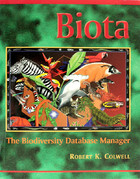
\includegraphics[scale=0.5]{images/Biota}
\par\end{center}
\begin{itemize}
\item Initial attempts at specimen level databasing failed.
\item All data lost due to hardware failures / ineffective back-up procedures
\end{itemize}

\lyxframeend{}\lyxframe{Progress Towards Digitisation}

\begin{center}

\includegraphics[scale=0.4]{images/BioLink}
\par\end{center}
\begin{itemize}
\item {}``Biodiversity Information Management System'' provided free by
CSIRO, Australia

\begin{itemize}
\item development and support discontinued in 2005
\item however, BioLink has recently been reborn as an \href{http://code.google.com/p/biolink/}{open source project}
\end{itemize}
\item written in Visual Basic 6/C++ and sits on top a MicroSoft SQL Server
database
\item typically run in client / server mode on a LAN or Internet
\end{itemize}

\lyxframeend{}\lyxframe{Current Status of Digitisation}

\begin{center}

\includegraphics[scale=0.4]{images/BioLink}
\par\end{center}
\begin{itemize}
\item All pinned specimens have been given a globally unique identifier
(GUID) and each has a BioLink record
\end{itemize}

\lyxframeend{}\lyxframe{Desirable Features for an Online Collection Database}
\begin{itemize}
\item Free and open source 
\item Reliable data security / backup 
\item Flexible data security (user permissions) 
\item Web browser used for data entry and information delivery
\item Specimen records compliant with Darwin Core 
\item Storage for images, bibliographic data, informal notes, etc.
\item Data shared via GBIF
\end{itemize}

\lyxframeend{}\lyxplainframe{}

\includepdf[pages={14}]{ScratchpadTrainingIntroOpt}


\lyxframeend{}\lyxplainframe{}

\includepdf[pages={15}]{ScratchpadTrainingIntroOpt}


\lyxframeend{}\lyxplainframe{}

\includepdf[pages={16}]{ScratchpadTrainingIntroOpt}


\lyxframeend{}\lyxplainframe{}

\includepdf[pages={17}]{ScratchpadTrainingIntroOpt}


\lyxframeend{}\lyxframe{Web 2.0 and Social Networking to the Rescue}


\lyxframeend{}\lyxframe{EOL and Scratchpads}

EOL vs ScratchPads; both Drupal; both hosted/maintained for free


\lyxframeend{}\section*{Scratchpads}


\lyxframeend{}\section*{Evaluation Results}


\lyxframeend{}\section*{Summary}


\lyxframeend{}\lyxframe{Dislikes}

\begin{center}

\includegraphics[scale=0.4]{images/cat-turntable-20110927-103305}
\par\end{center}

\begin{center}
ScratchPads
\par\end{center}

\begin{center}
The Name is Lame
\par\end{center}


\lyxframeend{}\lyxframe{Summary}
\begin{itemize}
\item The \textcolor{red}{first main message} of your talk in one or two
lines.
\item The \textcolor{red}{second main message} of your talk in one or two
lines.
\item Perhaps a \textcolor{red}{third message}, but not more than that.
\end{itemize}


\appendix

\lyxframeend{}\section*{Appendix}


\lyxframeend{}\subsection*{For Further Reading}


\lyxframeend{}\lyxframe{[allowframebreaks]For Further Reading}

\beamertemplatebookbibitems
\begin{thebibliography}{References}
\bibitem{Author1990}A. Author. \newblock\emph{Handbook of Everything}.\newblock
Some Press, 1990.\beamertemplatearticlebibitems

\bibitem{Someone2002}S. Someone.\newblock On this and that\emph{.}
\newblock\emph{Journal on This and That}. 2(1):50--100, 2000.

\end{thebibliography}

\lyxframeend{}
\end{document}
